
%%%%%%%%%%%%%%%%%%%%%%%%%%%%%%%%%%%%%%%%%%%%%%%%%%%%%%%%%%%%%%%%%
\section{Aufgabenstellung}
%%%%%%%%%%%%%%%%%%%%%%%%%%%%%%%%%%%%%%%%%%%%%%%%%%%%%%%%%%%%%%%%%
Der Vollständigkeit wegen wird hier noch einmal in eigenen Worten die Aufgabenstellung wiedergegeben.\\

Betrachtet wird eine Methan-Luft-Diffusionsflamme. Der Versuchsaufbau besteht aus zwei gegeneinander gerichteten Einlässen. Gravitationseffekte werden vernachlässigt, sodass ohne Beschränkung der Allgemeinheit Luft als von oben anströmend angenommen werden kann, siehe \autoref{fig:stream}
\begin{figure}[H]
    \begin{center}
        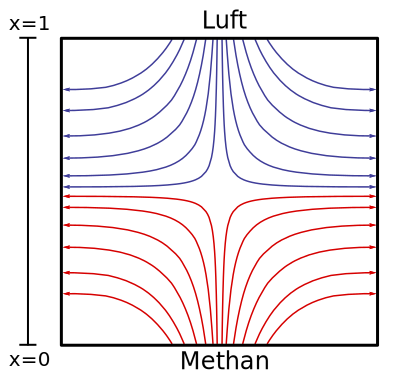
\includegraphics[width=0.4\linewidth]{stream}
    \end{center}
    \caption{Zu simulierender Versuchsaufbau mit qualitativ eingezeichneten Strömungsfeld}
    \label{fig:stream}
\end{figure}

Mit Hilfe des am Institut für Numerische Thermofluiddynamik (\gls{NTFD}) der Technischen Universität Bergakademie Freiberg (\gls{TUBAF}) entwickelten universellen laminaren Flammenlösers (\gls{ULF}) soll der Versuchsaufbau aus \autoref{fig:stream} simuliert und die Ergebnisse ausgewertet werden. Dabei sollen zwei verschiedene Lösungsmethoden angewandt werden: Eine Lösung im physikalischen Raum, also über den Ort diskretisiert und eine Lösung mittels Flamelets.

\begin{sloppypar} % to better break \lstinline (allows larger word distances
\begin{enumerate}
    \item Für die Simulation im physikalischen Raum soll das mit \gls{ULF} mitgelieferte Beispielsetup \lstinline!oppdifJet! benutzt werden. Für diese Konfiguration sind folgende Dinge durchzuführen
    \begin{enumerate}
        \item \label{itm:ople1-1}
        Trage die maximale Temperatur \gls{T_max} verschiedener Konfigurationen über die skalare Dissipationsrate bei stöchiometrischer Mischung \gls{chi_st} auf; z.B. durch Variation der Einströmgeschwindigkeiten.

        \item \label{itm:ople1-3}
        Trage die Temperatur \gls{T} und die Massenbrüche $Y_{\mathrm{CO}}$, $Y_{\mathrm{CO}_2}$, $Y_{\mathrm{H}_2}$, $Y_{\mathrm{H}_2O}$, $Y_{\mathrm{OH}}$ über den Ort \gls{x} für 5 verschiedene \gls{chi_st} auf (5 Plots) und vergleiche diese.

        \item \label{itm:ople1-4}
        Trage die skalare Dissipationsrate \gls{chi} über den Mischungsbruch \gls{Z} auf und vergleiche den Verlauf mit der analytischen Lösung, vgl. \autoref{eq:chianal}. Dies ist für 5 verschiedene \gls{chi_st} durchzuführen.

        \item \label{itm:ople1-5}
        Trage die maximale Temperatur aus \ref{itm:ople1-1} über die Fortschrittsvariable $\gls{PV}:=Y_\mathrm{CO}+Y_{\mathrm{CO}_2}$ auf

        \item \label{itm:ople1-6}
        Trage die Massenbrüche aus \ref{itm:ople1-3} über die in \ref{itm:ople1-5} definierte Fortschrittsvariable für 5 verschiedene \gls{chi_st} auf.

        \item \label{itm:ople1-7}
        Trage \gls{Z_Bilger} über \gls{Z} für 5 verschiedene \gls{chi_st} auf
    \end{enumerate}
    \item Nun soll die Simulation mittels Flamelets für $\mathrm{Le}=1$ mit dem Setup \lstinline!flameletLe1! durchgeführt werden. Wiederhole mit den so erhaltenen Werten Aufgabe~\ref{itm:ople1-1} bis \ref{itm:ople1-6}
    \item Wiederhole alle obigen Aufgaben für ein mixture averaged Diffusionsmodell, also $\mathrm{Le}\neq 1$. Für Flamelets ist das Beispielsetup \lstinline!flameletLeVar! zu nutzen. Da für $\mathrm{Le}\neq 1$ $Z_\mathrm{st}$ nicht eindeutig definiert ist, ist $Z_\mathrm{st}$ aus $\mathrm{Le}=1$ zu übernehmen.
\end{enumerate}
\end{sloppypar}
